% Tool-competition review draft, exploratory weight edits added 2026-11-03.
% Original PKP2 seed13 epoch4: 8048 updates; checkpoint identity unchanged.
% All measurements are reused; external figure asset is included in the review bundle.
\documentclass[10pt,conference]{IEEEtran}
\usepackage[T1]{fontenc}
\usepackage{amsmath,amssymb,booktabs,array,balance,graphicx}
\usepackage[hyphens]{url}
\usepackage[hidelinks]{hyperref}
\hypersetup{pdftitle={PairKD: A Two-Layer CodeBERT Model for Joint Weakness and SATD Classification},pdfauthor={Xin Xu and Jun Yu}}
\title{PairKD: A Two-Layer CodeBERT Model for\\Joint Weakness and SATD Classification}
\IEEEoverridecommandlockouts
\author{
\IEEEauthorblockN{Xin Xu}
\IEEEauthorblockA{Department of Automation\\
University of Science and Technology of China\\
Hefei, Anhui, China\\
xuxin123122@mail.ustc.edu.cn}
\and
\IEEEauthorblockN{Jun Yu\textsuperscript{*}}
\IEEEauthorblockA{Department of Automation and\\
Institute of Advanced Technology\\
University of Science and Technology of China\\
Hefei, Anhui, China\\
harryjun@ustc.edu.cn}
\thanks{*Corresponding author: Jun Yu (harryjun@ustc.edu.cn).}
}
\begin{document}
\maketitle

\begin{abstract}
PairKD classifies Weakness and MAT using code/comment views packed within 512 tokens and a shared two-layer CodeBERT encoder. A trained teacher supplies initialization and Bernoulli distillation targets; only the student is deployed. PKP2 (seed13, epoch4) has 53.77 million parameters and achieves Weakness/MAT/Mean F1 of .892311/.924528/.908419 at previously public-fitted thresholds. Its Tesla T4 reference score is .908788, versus .907850/.907252 for two narrow three-layer candidates. N13 has higher Mean F1 (.910578), offset by longer measured forward time. We document 15 actual T4 configurations and their training/threshold policies. Exposed public data and single-pass timing do not establish hidden-test performance.
\end{abstract}
\begin{IEEEkeywords}
CodeBERT, knowledge distillation, model compression, multitask classification, self-admitted technical debt.
\end{IEEEkeywords}

\section{Introduction}
The NLBSE'27 competition requires one model to classify a Function for Weakness and the MAT annotation used as its self-admitted technical debt (SATD) target~\cite{competition,madewic}. The predicted vector is [Weakness,MAT]; the labels are independent, so an instance may have neither, either, or both. The primary predictive metric averages task F1, while the reference ranking also rewards runtime and computational cost.

PairKD initializes a shallow CodeBERT~\cite{codebert} student from a trained teacher. The submission uses original PKP2 (seed13, epoch4), selected over PKP3 in paired T4 tests and retained after comparison with narrow three-layer candidates. Table~\ref{tab:configurations} explains the model IDs.

Code--comment separation and distillation have prior work~\cite{vulsatd,hinton,majeed}. Our contribution is a concrete compact tool configuration, its preprocessing and training procedure, and measured task-level accuracy--cost outcomes. The evaluation reports actual Tesla T4 measurements and distinguishes ranking metrics from chosen operating points.

\begin{figure*}[t]
\centering
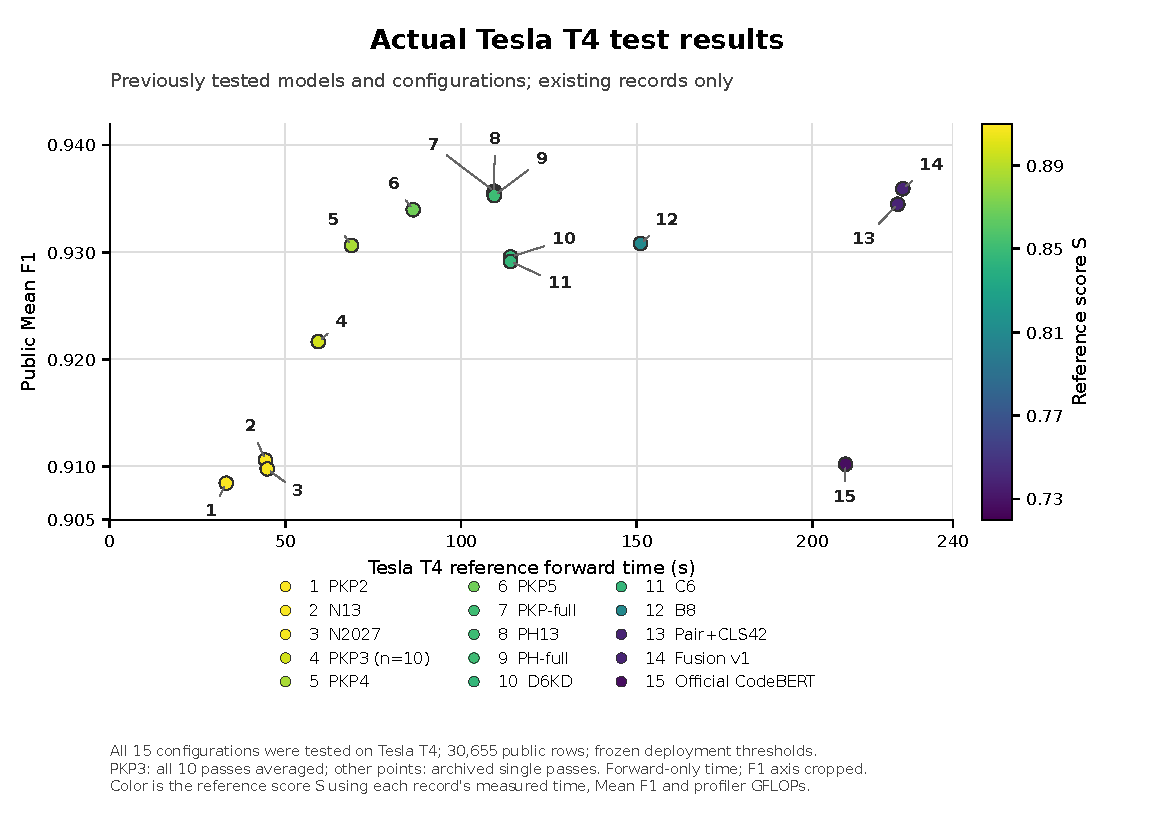
\includegraphics[width=\textwidth,trim=0 47 0 51,clip]{figures/t4_all_existing_models.pdf}
\caption{Actual Tesla T4 results for 15 previously tested checkpoints/configurations on 30,655 public-validation rows. Numbers map to Table~\ref{tab:configurations} and the model key inside the plot; color is the reference score computed with each record's profiler-reported GFLOPs. All configurations were measured on Tesla T4 using their frozen deployment thresholds. PKP3 uses the mean of all ten accepted passes; other plotted records are archived single passes. The F1 axis is cropped. Training and threshold policies are described in the text; these are public-validation results.}
\label{fig:t4overview}
\end{figure*}


\begin{table*}[t]
\centering
\caption{Configurations and actual T4 scores for the 15 points in Fig.~\ref{fig:t4overview}. All encoders use hidden size 768 and 12 attention heads. Rows/epochs exclude inherited supervision. $S$ (Eq.~3) combines Mean F1, time and GFLOPs. All scores are from Tesla T4 measurements at the frozen operating points.}
\label{tab:configurations}
\small
\setlength{\tabcolsep}{4pt}
\begin{tabular}{@{}rlrrrllrrrr@{}}
\toprule
No. & Record ID & Layers & FFN & Params (M) & Encoder start & Loss & Train rows & Epochs & Seed & T4 $S$\\
\midrule
1 & PKP2 & 2 & 3072 & 53.77 & Pair teacher & BCE+KD & 193,124 & 4 & 13 & 0.908788\\
2 & N13 & 3 & 1536 & 53.78 & Pruned grouped Pair & BCE+KD & 171,668 & 4 & 13 & 0.907850\\
3 & N2027 & 3 & 1536 & 53.78 & Pruned grouped Pair & BCE+KD & 171,668 & 4 & 2027 & 0.907252\\
4 & PKP3 & 3 & 3072 & 60.86 & Pair teacher & BCE+KD & 193,124 & 4 & 13 & 0.896663\\
5 & PKP4 & 4 & 3072 & 67.95 & Pair teacher & BCE+KD & 193,124 & 4 & 13 & 0.885356\\
6 & PKP5 & 5 & 3072 & 75.04 & Pair teacher & BCE+KD & 193,124 & 4 & 13 & 0.869031\\
7 & PKP-full & 6 & 3072 & 82.12 & Pair teacher & BCE+KD & 214,586 & 4 & 13 & 0.850643\\
8 & PH13 & 6 & 3072 & 82.12 & Pair teacher & BCE & 193,124 & 4 & 13 & 0.850544\\
9 & PH-full & 6 & 3072 & 82.12 & Pair teacher & BCE & 214,586 & 4 & 13 & 0.850394\\
10 & D6KD & 6 & 3072 & 82.12 & Raw supervised & BCE+KD & 193,124 & 2 & 13 & 0.846031\\
11 & C6 & 6 & 3072 & 82.12 & Raw supervised & BCE & 193,124 & 2 & 13 & 0.845785\\
12 & B8 & 8 & 3072 & 96.30 & Raw supervised & BCE & 193,124 & 2 & 13 & 0.809758\\
13 & Pair+CLS42 & 12 & 3072 & 124.65 & Raw supervised & BCE & 193,124 & 2 & 42 & 0.738061\\
14 & Fusion v1 & 12 & 3072 & 124.65 & Raw supervised & BCE & 193,124 & 2 & 42 & 0.738639\\
15 & Official CodeBERT & 12 & 3072 & 124.65 & Published & --- & --- & --- & --- & 0.726455\\
\bottomrule
\end{tabular}

\smallskip
\begin{minipage}{\textwidth}
\footnotesize
\textit{Reading the IDs.}
PKP2/3/4/5 are Pair-initialized, Pair-teacher KD students with the stated depth.
PKP-full is a \emph{six-layer} full-TRAIN refit; PH denotes the Pair-initialized hard-label control.
N13/N2027 are \emph{three-layer} narrow-FFN models; 13/2027 denote seeds.
D6KD/C6/B8 start from a supervised raw-Function encoder; D6KD adds Pair-teacher KD.
Pair+CLS42 uses paired input and first-token classification; Fusion v1 uses task-specific code/comment gates.
Pair teacher is the historical 12-layer seed42 model, whereas grouped Pair is rebuilt on 171,668 TRAIN rows.
BCE is weighted binary cross-entropy; BCE+KD is the objective in Eqs.~(1)--(2).
The official baseline uses its published checkpoint; upstream training fields are not reconstructed (---).
\end{minipage}
\end{table*}

\section{Classifier and Preprocessing}
\subsection{Inputs from Function}
The only model input is the supplied Function string. Project names, filepaths and labels are not features. A fixed lexical extractor derives code and comment views, recognizing line/block comments while preserving quoted strings and escapes. Its hash-comment branch excludes recognized C preprocessor directives. Comment delimiters are normalized without external text; this procedure is not a complete language parser.

The tokenizer encodes both views without individual special tokens and packs
\[
 \texttt{<s> code </s> </s> comment </s>}.
\]
Four positions hold special tokens. Within the 512-token limit, up to 96 tokens are initially reserved for comments, then code fills the available budget. Remaining capacity is returned to comment tokens and then code tokens. Each view retains its prefix; 96 is an initial reservation, not a universal comment cap. Without comments, the packer uses code and two special tokens. Evaluation right-pads to width 512 and preserves instance order.

\subsection{Shared shallow encoder}
The two-layer PairKD student (PKP2) copies embeddings and teacher layers [0,11] into a two-layer encoder with hidden size 768, 12 attention heads and feed-forward network (FFN) width 3072. Fresh seed13 linear heads map the first-token representation to logits in [Weakness,MAT] order. Sigmoid is applied independently to each output. The checkpoint has 53,771,526 parameters, including legacy pooler/gate tensors whose outputs are unused by the active CLS decision branch. They are retained to preserve the measured state dictionary.

The source teacher, Pair+CLS42, is a supervised 12-layer CodeBERT model with paired code/comment input and first-token (CLS) classification; 42 denotes its training seed. Its logits are exported for training rows only. Neither teacher weights nor optimizer state are needed by the deployed tool. The general inference entry accepts Function strings or label-free JSONL, preserves indices and duplicate rows, and returns FP32 probabilities and binary predictions.

\section{Training and Tuning}
\subsection{Partition and initialization}
Official TRAIN contains 214,586 instances. The original deterministic internal split assigns 193,124 to student updates and 21,462 to validation. The Pair+CLS42 teacher inherits an earlier raw-input supervised CodeBERT warm start, is trained on the fixed training partition, and is selected using internal validation. Student encoder initialization is therefore supervised rather than teacher-independent.

Cached logits are indexed for the 193,124 training rows. Both tasks use that same teacher; no teacher forward runs inside the student update loop. Training fixes four epochs and the epoch4 endpoint, retaining 8,048 optimizer updates. Other checkpoints are diagnostic, and the measured package is not a full-TRAIN refit.

\subsection{Objective and optimization}
The hard objective averages binary cross-entropy (BCE) across tasks, with positive weights 2.1517589 for Weakness and 59.6545219 for MAT. For task $j$,
\[
 p^s_j=\sigma(z^s_j/T),\quad p^t_j=\sigma(z^t_j/T),\qquad T=2.
\]
The student minimizes
\begin{align}
 \mathcal{L}_{\mathrm{KD}}&=\tfrac12\sum_{j=1}^{2}
 D_{\mathrm{KL}}\!\left(\mathrm{Ber}(p^t_j)\,\|\,\mathrm{Ber}(p^s_j)\right),\\
 \mathcal{L}&=\tfrac12\mathcal{L}_{\mathrm{BCE}}+
             \tfrac12T^2\mathcal{L}_{\mathrm{KD}}.
\end{align}
Both Bernoulli outcomes are included, independently of the other label. Teacher targets are detached; the KL term receives no class weights.

AdamW uses learning rate $3\times10^{-5}$, weight decay .01, gradient clipping at 1, and linear warmup/decay with 482 warmup updates. Microbatch 12 and eight accumulation steps give nominal batch 96; the last window contains 68 instances. Forwards use BF16 and logits/loss use FP32. The artifact records seed13, the four epoch orders, initialization and checkpoint identity.

\subsection{Threshold policy}
Model configurations are screened on internal validation, followed by public-validation deployment comparison. The selected two-layer student's packaged thresholds were fitted independently by task on the public split before these T4 runs: approximately [.59,.97], stored in float32 and applied with $\geq$. These exposed data must not be presented as an untouched test set. The N13/N2027 thresholds are approximately [.79,.84]/[.85,.91], previously fitted on grouped CAL. Table~\ref{tab:metrics} compares these frozen policies with fixed .5 using the same saved probabilities, without new fitting. No policy uses hidden labels.

\section{Evaluation and Configuration Trade-offs}
\subsection{Reference protocol}
Our student training and internal CAL/AUDIT evaluation used RTX 4090 GPUs. The public deployment results in Fig.~\ref{fig:t4overview} and Tables~\ref{tab:configurations}--\ref{tab:single} were measured on Tesla T4.

The public split contains 30,655 instances. T4 inference uses FP16 autocast, scaled dot-product attention (SDPA), FP32 sigmoid, batch 600 and global width 512. There are 52 batches, with a tail of 55. Two timed forwards per batch give 104 formal calls; elapsed time and profiler GFLOPs are divided by two. One synthetic batch 600 preflight per pass is excluded from scoring.

The timer begins after host-to-device transfer and includes the two forwards and their profiler context. Model loading, extraction/tokenization, sigmoid, output transfer and metrics are excluded: this is forward-only, not end-to-end latency. Supported-event profiler GFLOPs do not establish complete accounting for fused SDPA. Raw probabilities and essential metadata are saved before reporting; recovery does not repeat completed inference.

The adopted reference formula is
\begin{align}
 S&=.6\overline{F_1}+.2\max(1-t/1000,0)\nonumber\\
  &\quad+.2\max(1-g/3{,}000{,}000,0),
\end{align}
with $t$ in seconds and $g$ in GFLOPs. Scores are local reference values, not organizer-confirmed hidden ranks. The public prose describes ten measurements, whereas the archived executable references use two forwards per batch and divide by two. We preserve the adopted source and disclose this unresolved difference.

\subsection{Public classification results}
\begin{table}[t]
\centering
\caption{Public metrics from the same saved outputs: frozen-policy precision ($P$), recall ($R$) and F1 versus fixed-.5 F1. PKP2 uses public-fit thresholds; N uses CAL-fit thresholds. Students use $\geq$; the baseline uses $>.5$ under both policies.}
\label{tab:metrics}
\small
\setlength{\tabcolsep}{3pt}
\begin{tabular}{@{}llrrrr@{}}
\toprule
Model & Output & \multicolumn{3}{c}{Frozen policy} & Fixed .5\\
\cmidrule(lr){3-5}
 & & $P$ & $R$ & F1 & F1\\
\midrule
Baseline & Weakness & .942651 & .935336 & .938979 & .938979\\
         & MAT      & .978261 & .801980 & .881393 & .881393\\
         & Mean     & .960456 & .868658 & .910186 & .910186\\
PKP2     & Weakness & .871856 & .913749 & .892311 & .889377\\
         & MAT      & .982183 & .873267 & .924528 & .896552\\
         & Mean     & .927019 & .893508 & .908419 & .892964\\
N13      & Weakness & .901000 & .905392 & .903191 & .894642\\
         & MAT      & .965066 & .875248 & .917965 & .909651\\
         & Mean     & .933033 & .890320 & .910578 & .902147\\
N2027    & Weakness & .922268 & .881715 & .901536 & .895234\\
         & MAT      & .965066 & .875248 & .917965 & .904082\\
         & Mean     & .943667 & .878481 & .909750 & .899658\\
\bottomrule
\end{tabular}
\end{table}

Table~\ref{tab:metrics} separates threshold policy from the saved model outputs. PKP2 has lower Weakness F1 and higher MAT F1 than the baseline at the frozen points. N13 leads the student comparison at fixed .5. Using the same recorded forward costs, fixed-.5 scores for PKP2/N13/N2027 are .899515/.902791/.901197; frozen PKP2 retains the highest reported deployment score (.908788). These diagnostics do not change the selected model or thresholds. Different training and threshold sources preclude an isolated architecture comparison.

Saved-probability Weakness AP is .961729 for PKP2 versus .966702/.968315 for N13/N2027; MAT AP is .888405 versus .890836/.891092. AP is non-interpolated average precision, distinct from trapezoidal PR area. Higher AP does not ensure higher frozen-threshold F1 or better calibration. The N models have equal MAT confusion totals but differ on eight negative decisions. Complete PR and threshold-sensitivity data are retained; no new optimum was selected.

\subsection{Tesla T4 deployment comparison}
\begin{table}[t]
\centering
\caption{Tesla T4 measurements with one whole-public pass per candidate; forward-only costs, frozen thresholds, $n=1$. GFLOPs are profiler-reported.}
\label{tab:single}
\small
\begin{tabular}{@{}lrrrr@{}}
\toprule
Model & Mean F1 & Seconds & GFLOPs & $S$\\
\midrule
PKP2  & .908419 & 33.16 & 444,468.63 & .908788\\
N13   & .910578 & 44.32 & 444,492.74 & .907850\\
N2027 & .909750 & 44.82 & 444,492.74 & .907252\\
\bottomrule
\end{tabular}
\end{table}

Table~\ref{tab:single} reports Tesla T4 measurements with PyTorch 2.11.0+cu130 and Transformers 5.16.1, in the fixed order PKP2/N13/N2027. All three raw outputs precede label-based reporting. N13 increases Mean F1 by .002158, but its measured time increases by 11.157 seconds; the reference score decreases by .000938. Near-equal reported GFLOPs do not imply equal latency. These single observations do not estimate timing variance or establish a stable ranking.

An earlier ten-pair PKP2/PKP3 campaign alternates their order, retaining all 20 passes and their 2,080 formal calls plus 20 preflights. Mean times are 39.87/59.36 seconds and mean scores .907447/.896663, with PKP2 winning 10/10 pairs. No fastest pass is selected; probabilities are identical within each candidate. These values summarize all ten paired rounds; Table~\ref{tab:single} reports the subsequent single-round comparison.

\subsection{Width--depth and historical comparisons}
The narrow-FFN student N uses three layers [0,6,11], hidden 768 and FFN 1536, totaling 53,776,902 parameters. Width/depth compression has prior work~\cite{dynabert}; N is an empirical configuration. It starts from an untrained three-layer student template; each layer retains 1536 FFN neurons ranked by the product of incoming-row and outgoing-column $L_2$ norms. Selected rows/biases and columns are physically copied, not masked. The two downstream seeds share the pruned initial encoder and use their matched fresh heads and training orders.

The grouped RTX 4090 experiments use 171,668 TRAIN, 21,459 calibration (CAL) and 21,459 audit (AUDIT) rows, rebuilt TRAIN-only teachers and 7,156 updates per student. Against matched two-layer FFN3072 BCE+KD controls (A13/A2027), N gains .009001/.008165 Mean F1 in five-fold CAL threshold cross-fitting on fixed probabilities. Weakness AP improves in both seeds; MAT AP falls in seed13 and rises in seed2027. At fixed-.5, average MAT F1 changes by $-.006539$. Depth, layer map and pruned initialization change together.

Figure~\ref{fig:t4overview} shows actual T4 results for the 15 configurations in Table~\ref{tab:configurations}, one record per configuration. PKP3 uses its ten-pass mean, PKP2/N their later single passes, and other points their historical measurements.

\subsection{Exploratory weight edits}
With GPT-6 Astra assistance, we made three label-informed weight edits without backpropagation using 10,809 historical internal rows: (1) a regularized Newton update to the Weakness head; (2) a pairwise ranking update to that edited head; and (3) a rank-one update to the original PKP2's final FFN projection with a penalty on MAT logit changes. On 10,653 comparison rows reused across rounds (RTX 3050 Laptop GPU), Mean F1 for original PKP2 and edits 1--3 was .902000/.902557/.902185/.902601 at frozen thresholds and .894284/.895086/.895106/.894807 at fixed .5. Weakness AP was .961777/.961776/.961516/.961807; MAT decisions were unchanged at both policies. Paired text-group bootstrap intervals for frozen-threshold Mean F1 differences versus the original all crossed zero. These exploratory edits leave the submission checkpoint and thresholds unchanged.

\section{Artifact and Validity}
The offline artifact includes the frozen checkpoint, tokenizer, configuration, thresholds, Function-only inference, provenance and Colab notebooks. Inference preserves row identity and duplicates and handles empty input. Private source supplies training, cache and tuning adapters; worker settings differ and exact checkpoint regeneration is unverified. Public release, source/model URLs, licenses and organizer-interface acceptance remain pending.

Public data and grouped CAL/AUDIT have development exposure. File and lexical grouping cannot exclude all near clones or shared projects, and some filepaths are missing. Student seeds share upstream supervision. Timing and AP do not establish hidden accuracy, label correctness or calibration.

\section{Conclusion}
PairKD provides a shared two-layer tool with frozen input handling, teacher-derived initialization and binary distillation. Higher Mean F1 from a deeper narrow configuration does not automatically offset its target-device latency. Actual T4 measurements and transparent policy/source reporting support the current PKP2 choice; final hidden ranking and public artifact release remain pending.

\begin{thebibliography}{7}
\bibitem{competition}
M.~Mock \emph{et al.}, \emph{The NLBSE'27 Tool Competition and Challenge},
official organizer-provided citation, 2027. Task/rules accessed
Oct.~9, 2026. [Online]. Available: \url{https://nlbse2027.github.io/tools/}
\bibitem{madewic}
M.~Mock, J.~Melegati, M.~Kretschmann, N.~E.~Diaz~Ferreyra, and B.~Russo,
\emph{MADE-WIC: Multiple Annotated Datasets for Exploring Weaknesses In Code},
in IEEE/ACM ASE, 2024, pp.~2346--2349, doi:~10.1145/3691620.3695348.
\bibitem{codebert}
Z.~Feng \emph{et al.}, \emph{CodeBERT: A Pre-Trained Model for Programming
and Natural Languages}, in Findings of EMNLP, 2020, pp.~1536--1547,
doi:~10.18653/v1/2020.findings-emnlp.139.
\bibitem{vulsatd}
B.~Russo, J.~Melegati, and M.~Mock, \emph{Leveraging Multi-Task Learning
to Improve the Detection of SATD and Vulnerability}, in IEEE/ACM ICPC,
2025, pp.~1--12, doi:~10.1109/ICPC66645.2025.00017.
\bibitem{hinton}
G.~Hinton, O.~Vinyals, and J.~Dean, \emph{Distilling the Knowledge in a
Neural Network}, arXiv:1503.02531, 2015.
\bibitem{majeed}
M.~A.~Majeed and A.~B.~Asim, \emph{Distilling Semantics: Efficient
Multi-label Code Comment Classification}, NLBSE 2026, conference
program and author manuscript, 2026.
\bibitem{dynabert}
L.~Hou \emph{et al.}, \emph{DynaBERT: Dynamic BERT with Adaptive Width
and Depth}, in Advances in Neural Information Processing Systems,
2020, arXiv:2004.04037.
\end{thebibliography}
\end{document}
